\section{Results}\label{sec:results}

\subsection{Training behaviour}\label{sec:res-training}

The network trained for $\trainSteps$ steps. The loss of Eq.~\eqref{eq:loss} fell from \trainFirstLoss{} at the first logged step to an average of \trainLastLoss{} over the last ten logged steps (Figure~\ref{fig:training}a), a decrease that the batch-to-batch variation of the trap sets makes noisy: the batches differ in the number of traps from one step to the next. The logged quantity that matters for the question is the spread after the last unrolled iteration, which the training script measures for the network
phases and, on the same batch, for random phases (Figure~\ref{fig:training}b). Over the last twenty logged steps the median spread after ten iterations is \trainSigNet{} percent for the network phases and \trainSigRand{} percent for random phases at the training freeze index $\nfix=3$: the network is not better than random phases at the end of the unrolled iteration on the training distribution, although it is better at the first iteration (\trainSigNetFirst{} against \trainSigRandFirst{} percent after iteration 1).
The advantage the loss rewards at the start is gone by iteration ten. On the held-out geometries the advantage after the first iteration is absent as well: the median spread after iteration 1 is \trNThreeOne{} percent for the network start and \trRTwelveOne{} percent for the random start (Table~\ref{tab:main} gives the other quantities).

\begin{figure}[t]
\centering
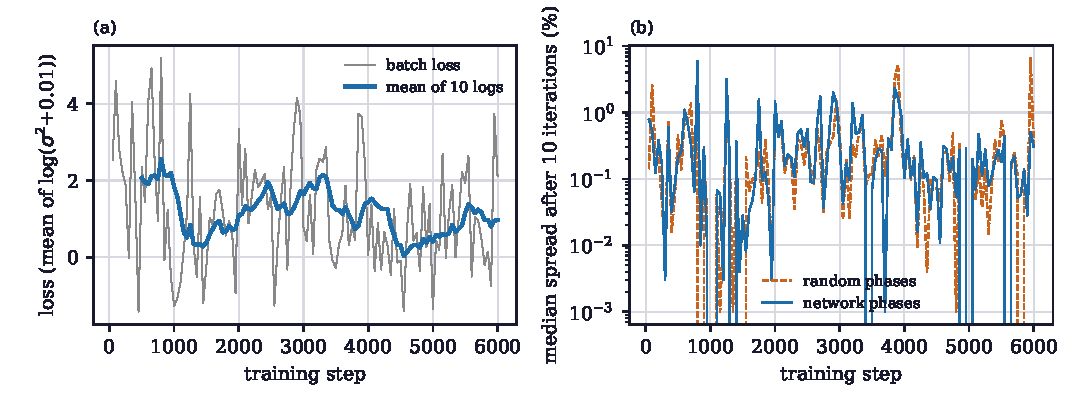
\includegraphics[width=\textwidth]{fig-training.pdf}
\caption{Training of the warm-start network: (a) loss of Eq.~\eqref{eq:loss} per logged step with a mean of ten logs; (b) median spread after the last unrolled iteration for the network phases and for random phases on the same training batches, per logged step, on a logarithmic axis.}
\label{fig:training}
\end{figure}

\subsection{Main comparison on held-out geometries}\label{sec:res-main}

Table~\ref{tab:main} gives the four phase-fixed WGS arms and the two published references on the $\nGeo$ held-out geometries ($\nSeeds$ seeds each, a budget of $\budget$ iterations). The published default (random start, $\nfix=12$) reaches 1 percent at a median of \itRTwelve{} iterations, with a tight spread (quartiles \itRTwelveQa{} to \itRTwelveQb) and \neverRTwelve{} percent of runs that do not reach it within the budget; the references are
slower or less reliable: the unweighted Gerchberg--Saxton iteration does not reach 1 percent within the budget on \neverMFour{} percent of the runs, and weighted GS reaches it at a median of \itMSix{} iterations (interval \itMSixLo{} to \itMSixHi), failing on \neverMSix{} percent of the runs. The candidate, the network start at $\nfix=3$, reaches 1 percent at a median of \itNThree{} iterations, with a 95\% bootstrap interval of \itNThreeLo{} to \itNThreeHi{}, and the ratio of the default's median to the candidate's is \ratioRoverN{} (interval \ratioRoverNLo{} to \ratioRoverNHi). The point estimate is below the required factor of two and the interval
includes values well below it; it also includes one, so the speed-up of the candidate over the default is not established at the 95\% level by this interval. The paired sign test over geometries gives the same reading: the candidate needs fewer iterations than the default on \signARN{} geometries and more on \signBRN{} ($\signTRN$ ties), $p=\signPRN$.

\begin{table}[t]
\centering\small
\resizebox{\textwidth}{!}{\begin{tabular}{@{}llrrrrr@{}}
\toprule
Start & $n_{\mathrm{fix}}$ & Median it. [95\% CI] & Q1--Q3 & Never (\%) & Final $\sigma$ (\%) & Efficiency \\
\midrule
random (engine default) & 12 & 14 [14, 14] & 13--15 & 6.1 & 0.00013 & 0.790 \\
random & 3 & 7.5 [6, 10.5] & 5--61 & 32.8 & 0.217 & 0.757 \\
network (candidate) & 3 & 8 [7, 17] & 5--61 & 34.8 & 0.216 & 0.756 \\
network & 12 & 14 [14, 14.5] & 13--15 & 4.5 & 0.000222 & 0.791 \\
Gerchberg--Saxton, random start & -- & 61 [61, 61] & -- & 100 & 16.3 & 0.821 \\
weighted GS, random start & -- & 30 [27, 36] & -- & 6.6 & 0.472 & 0.808 \\
\bottomrule
\end{tabular}
}
\caption{Iterations to a relative standard deviation of 1\% on the $\nGeo$ held-out geometries: median over geometries with a bootstrap 95\% interval, quartiles, the share of runs that never reach 1\% within \budget{} iterations, the median final spread $\relstd$ in percent and the median final efficiency, for the four arms of phase-fixed WGS and two published references from the random start.}
\label{tab:main}
\end{table}

The final quantities show the price of the early freeze, whatever the start. The final median spread is \finRTwelve{} percent at $\nfix=12$ and \finRThree{} (random) and \finNThree{} (network) percent at $\nfix=3$, and the final efficiency is \effmRTwelve{} at the default and \effmRThree{} and \effmNThree{} with the early freeze. The relative difference of the medians of the final efficiency between the candidate and the default is \effdNThree{} percent, between a random start with
the early freeze and the default \effdRThree{} percent, and between the candidate and the random start with the same freeze \effdNThreeRThree{} percent; the final uniformity median differs by \recUni{} percent in the committed record of the candidate. The candidate reproduces the committed record of its first evaluation (median \recMedModel{} against \recMedRandom{}, factor \recRatio{}, efficiency difference \recEff{} percent): the arms of this study differ from that evaluation by the network being read from its training checkpoint rather than from the exported graph.

\subsection{Outcome of the hypotheses}\label{sec:res-hyp}

H1 is not supported: the factor is \ratioRoverN{}, below $2$, and the interval \ratioRoverNLo{} to \ratioRoverNHi{} does not exclude no gain at all. H2 is not supported: the final efficiency of the candidate is \effdNThree{} percent from the default's, above the 1 percent allowed. H3 is met: the exported graph is \onnxBytes{} bytes. H4 is supported by the three arms of Section~\ref{sec:ablation}: a random start with the same early freeze gives a factor of \ratioRoverRThree{} (interval \ratioRoverRThreeLo{} to
\ratioRoverRThreeHi, sign test $p=\signPRRThree$) and the same efficiency loss, and the network at the default freeze index gives a factor of \ratioRoverNTwelve{}. Because H1 failed, the model is not released, and the slot of the product answers with the random start of the iteration.

Taken together, the acceptance test is failed on its first two clauses and passed on the third, which is the pattern of a start that is small and ineffective, not of a start that is large and inaccurate. The effect that remains with respect to the published default, the lower median iterations, is reproduced by the control without a network; the effect of the network beyond the control is not distinguishable from zero in any of the measured quantities, the median, the share of runs that converge, the final spread and the final efficiency.

\subsection{Convergence along the iterations}\label{sec:res-traces}

Figure~\ref{fig:traces} shows the median spread of each arm along the iterations, with the interquartile band across geometries. The curves of the two arms with the same freeze index are almost on top of each other: the two $\nfix=12$ arms follow the staircase of the default, with the spread at several percent until the freeze (\trRTwelveEleven{} percent at iteration 11 for the random start, \trNTwelveEleven{} for the network) and a drop at the first iteration after it
(\trRTwelveThirteen{} and \trNTwelveThirteen{} percent at iteration 13); the two $\nfix=3$ arms drop at iteration 4 (\trRThreeFour{} percent for the random start, \trNThreeFour{} for the network) and then flatten at a spread of about 0.4 percent. The plateau is why the $\nfix=3$ arms do not reach 1 percent on a third of the runs: for the median geometry the frozen phases allow 1 percent, for the geometries in the upper quartile they do not. Figure~\ref{fig:ecdf} shows the distribution of the iterations
over the geometries: the early-freeze arms have their first quartile at \itRThreeQa{} iterations and their third quartile at the cap, while the default has quartiles of \itRTwelveQa{} and \itRTwelveQb{}.

\begin{figure}[t]
\centering
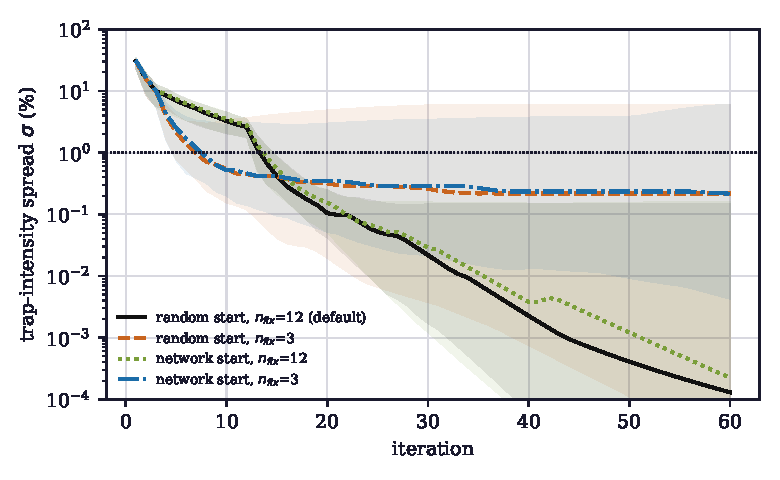
\includegraphics[width=0.78\textwidth]{fig-traces.pdf}
\caption{Median relative standard deviation of the trap intensities along the $\budget$ iterations of phase-fixed WGS on the $\nGeo$ held-out geometries, for the four arms (random or network start, $\nfix=3$ or $12$); the bands are the interquartile range across geometries and the dotted line is the 1\% threshold.}
\label{fig:traces}
\end{figure}

\begin{figure}[t]
\centering
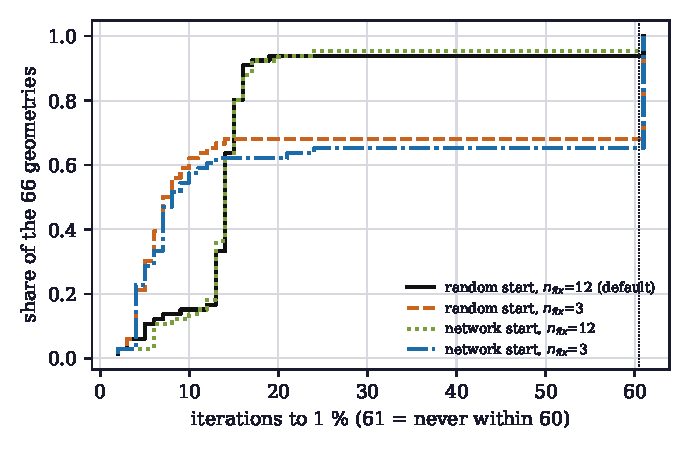
\includegraphics[width=0.62\textwidth]{fig-ecdf.pdf}
\caption{Empirical distribution of the iterations to 1\% over the $\nGeo$ held-out geometries for the four arms; the value $\budget+1$ marks the geometries that never reach 1\% within the budget, which is where the early-freeze arms leave about a third of the geometries.}
\label{fig:ecdf}
\end{figure}

\subsection{Geometry by geometry}\label{sec:res-paired}

Figure~\ref{fig:paired} compares the arms geometry by geometry. Against a random start with the same freeze index (Figure~\ref{fig:paired}a) the points lie on the diagonal: the network start needs the same number of iterations on \signTRThreeN{} of the $\nGeo$ geometries, fewer on \signARThreeN{} and more on \signBRThreeN{} (sign test $p=\signPRThreeN$), so if anything the network is slightly slower than the random start at $\nfix=3$, a difference that is not
distinguishable from none. Against the default (Figure~\ref{fig:paired}b) the network start needs fewer iterations on \signARN{} geometries and more on \signBRN{}, the latter being mostly geometries on which it does not converge at all. Of the \nGeo{} geometries, \capBoth{} reach the cap with both early-freeze arms, \capRNotN{} only with the random start and \capNNotR{} only with the network start. The medians separated by group are \genItRTwelve{} (random, $\nfix=12$), \genItRThree{} (random, $\nfix=3$) and \genItNThree{} (network, $\nfix=3$) on the generated geometries, and \benchItRTwelve{}, \benchItRThree{} and \benchItNThree{} on the six benchmark geometries.

\begin{figure}[t]
\centering
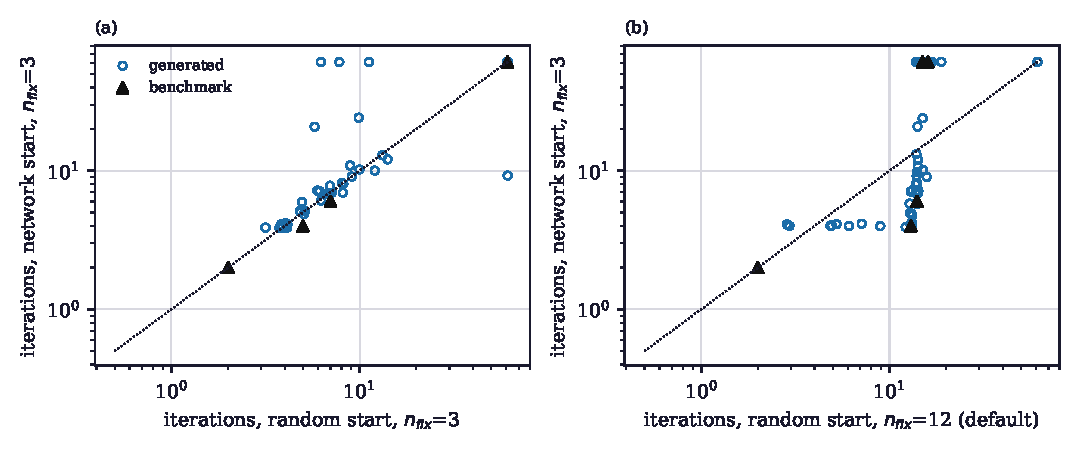
\includegraphics[width=\textwidth]{fig-paired.pdf}
\caption{Iterations to 1\% per held-out geometry, network start at $\nfix=3$ (vertical axis) against (a) the random start at $\nfix=3$ and (b) the random start at the default $\nfix=12$ (horizontal axis), logarithmic axes, with a small jitter for ties; circles are generated geometries, triangles the six benchmark geometries, the dotted line is equality and $\budget+1$ marks a run that never reaches 1\%.}
\label{fig:paired}
\end{figure}
